\section{Ejercicio E - Gráficas}

\subsection{Problema}

Represente en una misma gráfica $x(t)$, $y(t)$, $z(t)$ en función del tiempo. Represente $x(t)$ en función de $y(t)$. A la vista de los resultados, ¿quéconclusiones puede extraer sobre el movimiento de la partícula? Sin necesidad de ajustes, obtenga una estimación de la velocidad de arrastre de la partícula (también llamada de deriva) y de la frecuencia ciclotrón. Compare con los valores teóricos esperados.


\subsection{Resolución}

El código que resuelve este ejercicio se puede ver en \ref{code:ex5}.

\paragraph{Gráficas de los componentes de $\vec{r}(t)$}

A continuación está la gráfica de los componentes del vector de posición en función del tiempo.

\begin{figure}[H]
	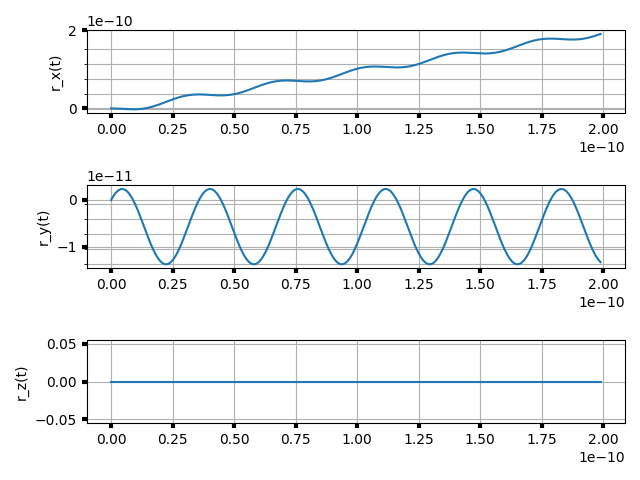
\includegraphics[width=\linewidth]{figures/no_rel_rx_ry_rz.png}
	\caption{Gráfica $r_x(t)$, $r_y(t)$, $r_z(t)$ en función de $t$}
	\label{fig:no_rel_x_y_z_t}
\end{figure}

\newpage 

\paragraph{Gráficas de $\vec{r}_x(t)$ y $\vec{r}_y(t)$}

A continuación está la gráfica de $r_x(t)$ en función de $r_y(t)$.

\begin{figure}[H]
	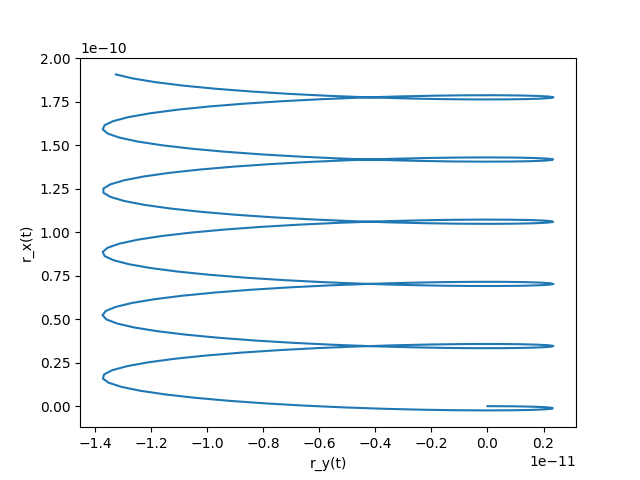
\includegraphics[width=\linewidth]{figures/no_rel_y_x.png}
	\caption{Gráfica $r_x(t)$ en función de $r_y(t)$}
	\label{fig:no_rel_y_x}
\end{figure}

\subsection{Discusión}

Las gráficas dejan claro que el ciclotrón tiene bien merecido su nombre, la partícula cargada, en este caso un electrón, acelerado en trayectoria de espiral, avanzando en dirección del eje-x.

La frecuencia angular ciclotrón es dada por:

$$
f = \frac{q}{m 2 \pi}B
$$

Por lo que $f \approx 3 \cdot 10^{10}$ y el periodo $T \approx 0.333 \cdot 10^{-10}$.

Vemos este periodo claramente presente en la figura \ref{fig:no_rel_x_y_z_t} para $\vec{r}_y(t)$ (la segunda fila). Es un poco menos evidente en la figura \ref{fig:no_rel_y_x}, pero si nos fijamos en el eje vertical (i.e: $\vec{r}_x(t)$) se puede percibir.

Si aproximamos la velocidad de deriva como: $\frac{\Delta \vec{r}_x(t)}{\Delta t}$, esto nos da: $v_{deriva} \approx \frac{2 \cdot 10^{-10}}{2 \cdot 10^{-10}} = 1$, que concuerda con el valor teórico dado por: $v_{deriva} = \frac{\vec{E} \times \vec{B}}{B^2} = (1, 0, 0)$. 